\chapter[Machine Learning]{Machine Learning}\label{c:tc4}

\section{Rationale of using machine learning}

Determining the energy level alignment of 2D perovskites presents a challenge due to the high computational cost of electronic structure calculation. Standard calculations using hybrid functionals and spin-orbital coupling on 2D perovskite unit cells with over 100 atoms make large-scale computations impractical. To address this challenge, our approach combines machine learning, frontier level calculation of isolated organic spacers, and electronic structure calculations of 2D perovskites progressively, each with increasing computational cost, to enhance the predictive power of our project. Initially, we calculate the frontier levels of isolated organic spacers to assess the potential for different energy level alignments. This initial step involves using organic descriptors as input feature and Gaussian calculation of frontier levels as output variable for a subset of molecules (generations 0-3, 3,000+ molecules) to train the machine learning model. This model is then used to predict the frontier levels of other molecules (generation 4, 30,000+ molecules). Subsequently, molecules with appropriate frontier levels are selected for more computationally intensive methods to calculate energy level alignment. By using the approach, we can overcome the computational challenges associated with determining the energy level alignment of 2D perovskites.

\section{Preprocessing and build model}
\subsection{Problem-specific descriptors}
\subsection{Model prediction}
\subsection{Model selection}

\section{Model performance}

\section{Model interpretation}

\section{DFT validation}

\begin{figure}[!ht]
\centering
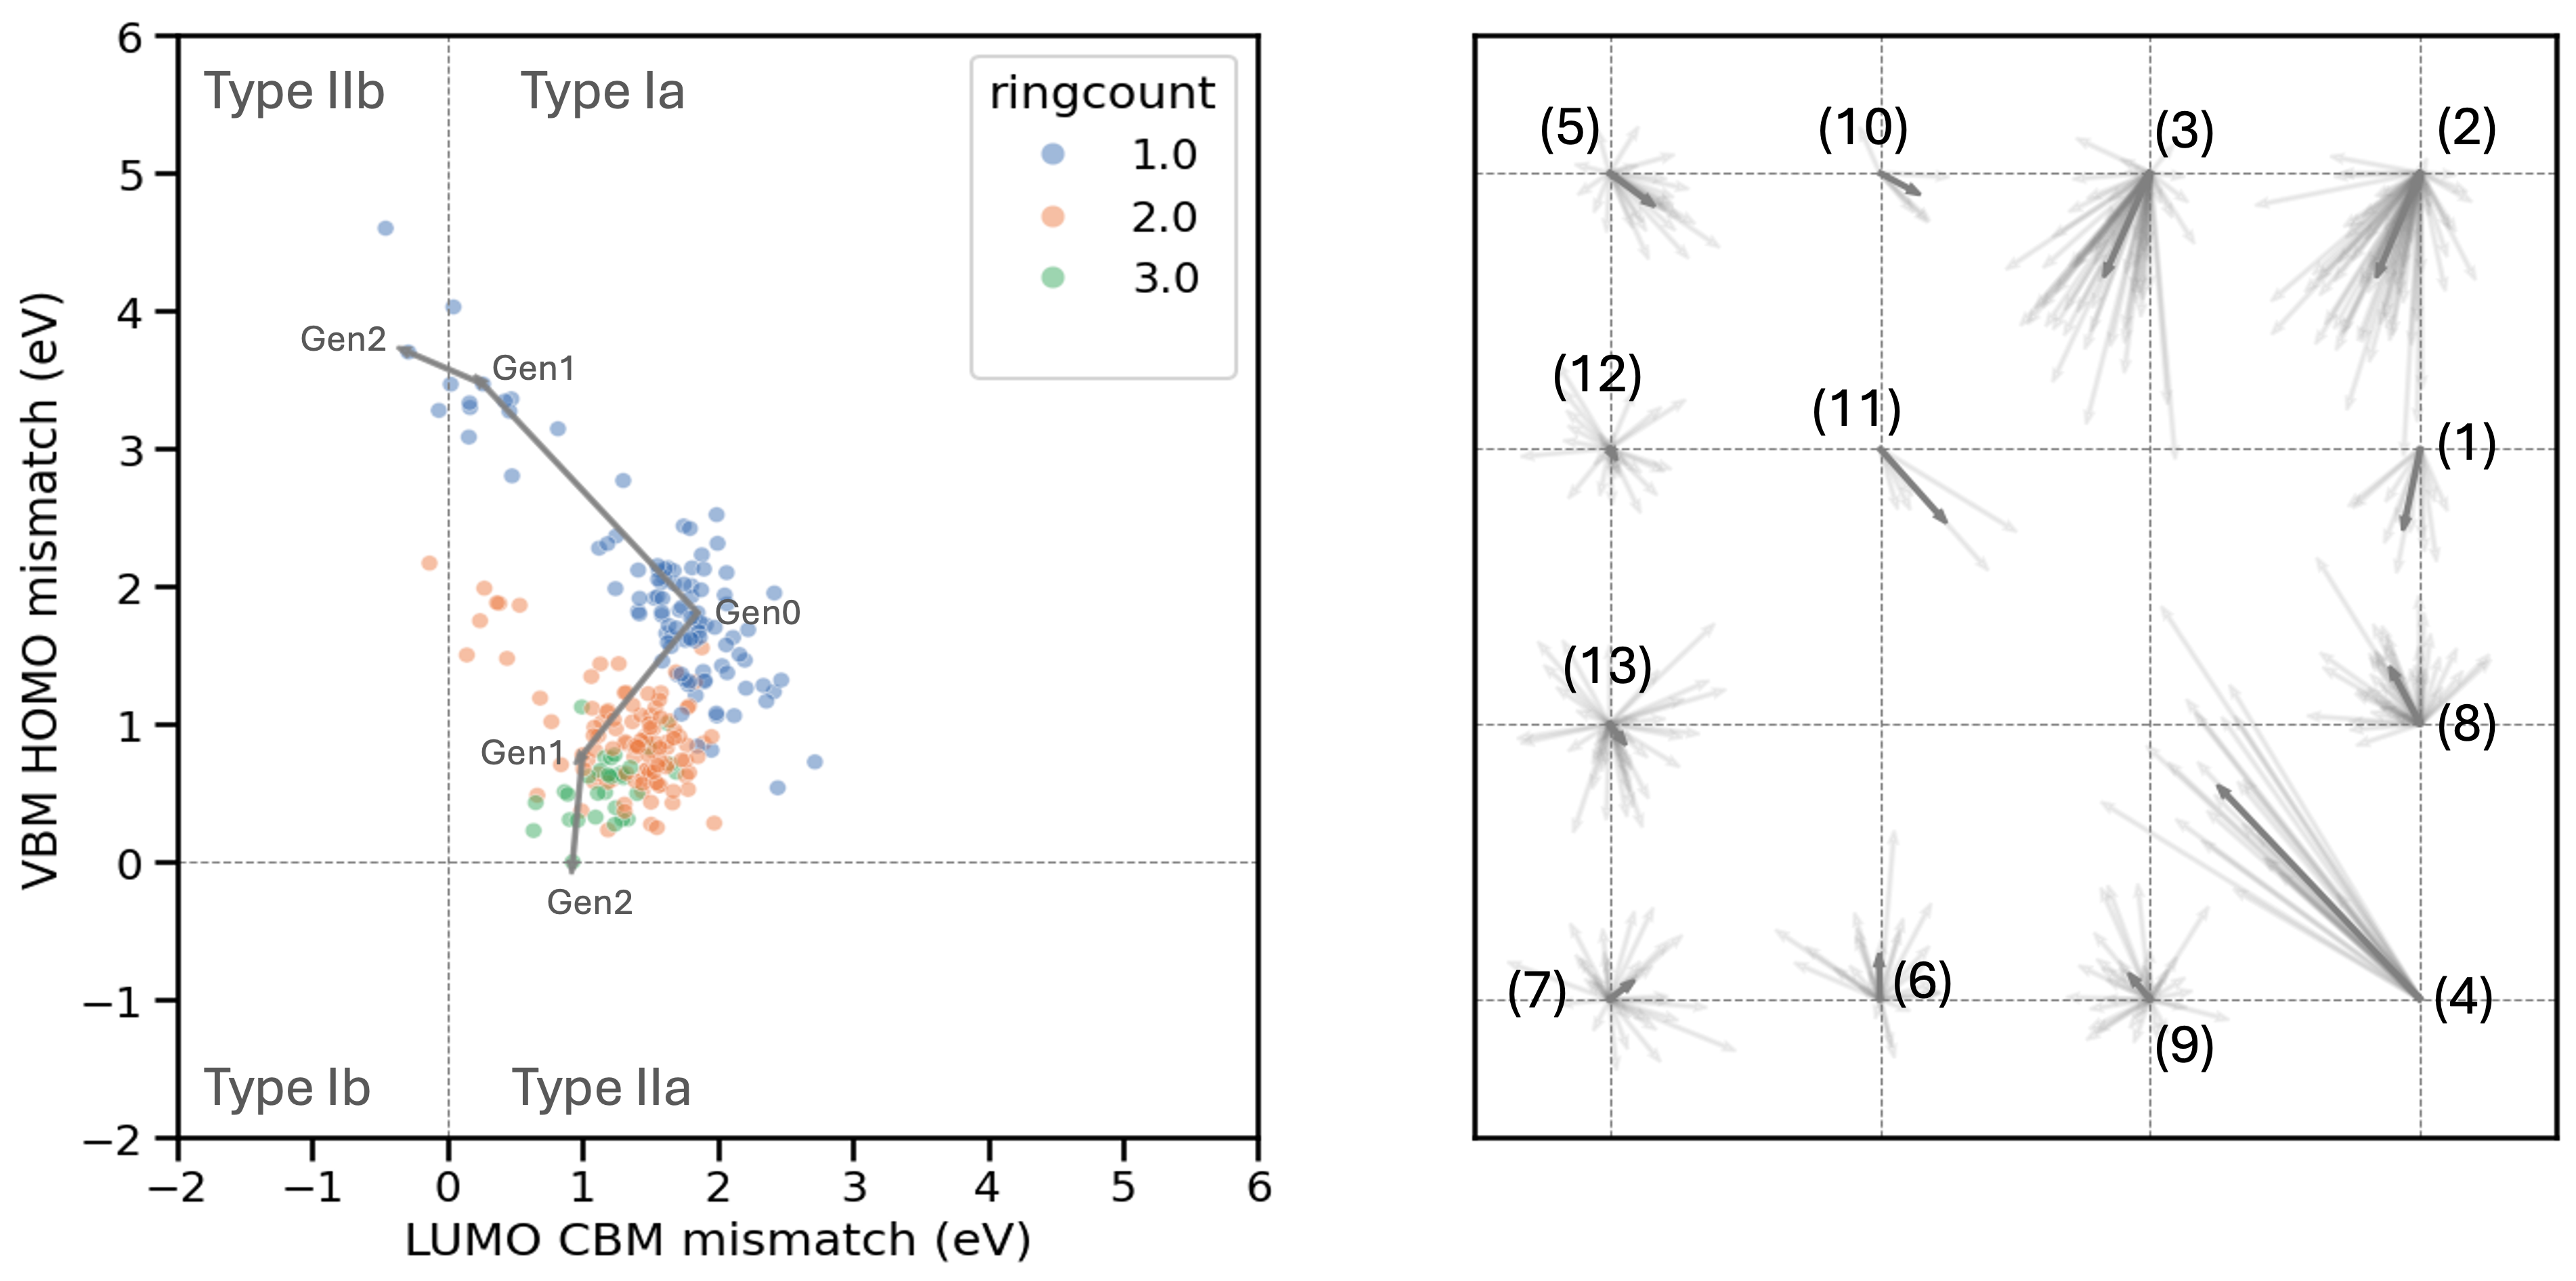
\includegraphics[width=\textwidth]{figures/machine-learning/machine-learning-1.png}
\caption[Energy level alignment and morphing pathways of DJ perovskites.]{Energy level alignment and morphing pathways of DJ perovskites. (a) Energy level alignment quadrant containing the energy level mismatch of organic spacers in generation 0-2 calculated by hybrid functional. Organic spacers are color coded by their number of rings. Morphing pathways for two example organic spacers are depicted (b) Impact of different types of morphing operations on the location of organic spacers in the energy level alignment quadrant.}
\label{f:machinelearning1}
\end{figure}

\begin{figure}[!ht]
\centering
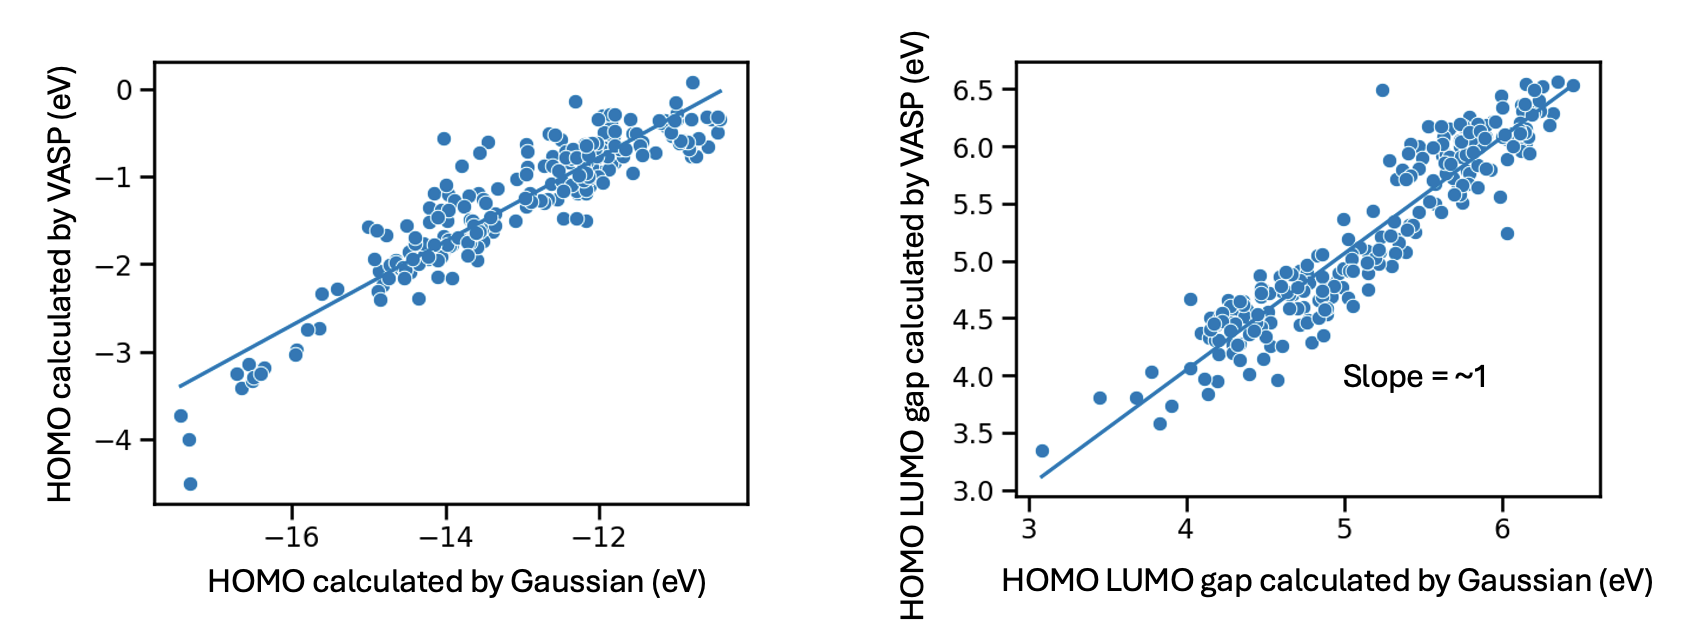
\includegraphics[width=\textwidth]{figures/machine-learning/machine-learning-2.png}
\caption[Comparison and correlation between organic frontier levels calculated using different methods.]{Comparison and correlation between organic frontier levels calculated using different methods. (a) Linear relationship between organic HOMO calculated in 2D perovskite structure using VASP and isolated organic spacer using Gaussian. (b) The organic HOMO-LUMO-gap is consistent between hybrid perovskite structure in VASP calculation and isolated organic spacer in Gaussian calculation.}
\label{f:machinelearning2}
\end{figure}



\clearpage
\begin{figure}[!ht]
\centering
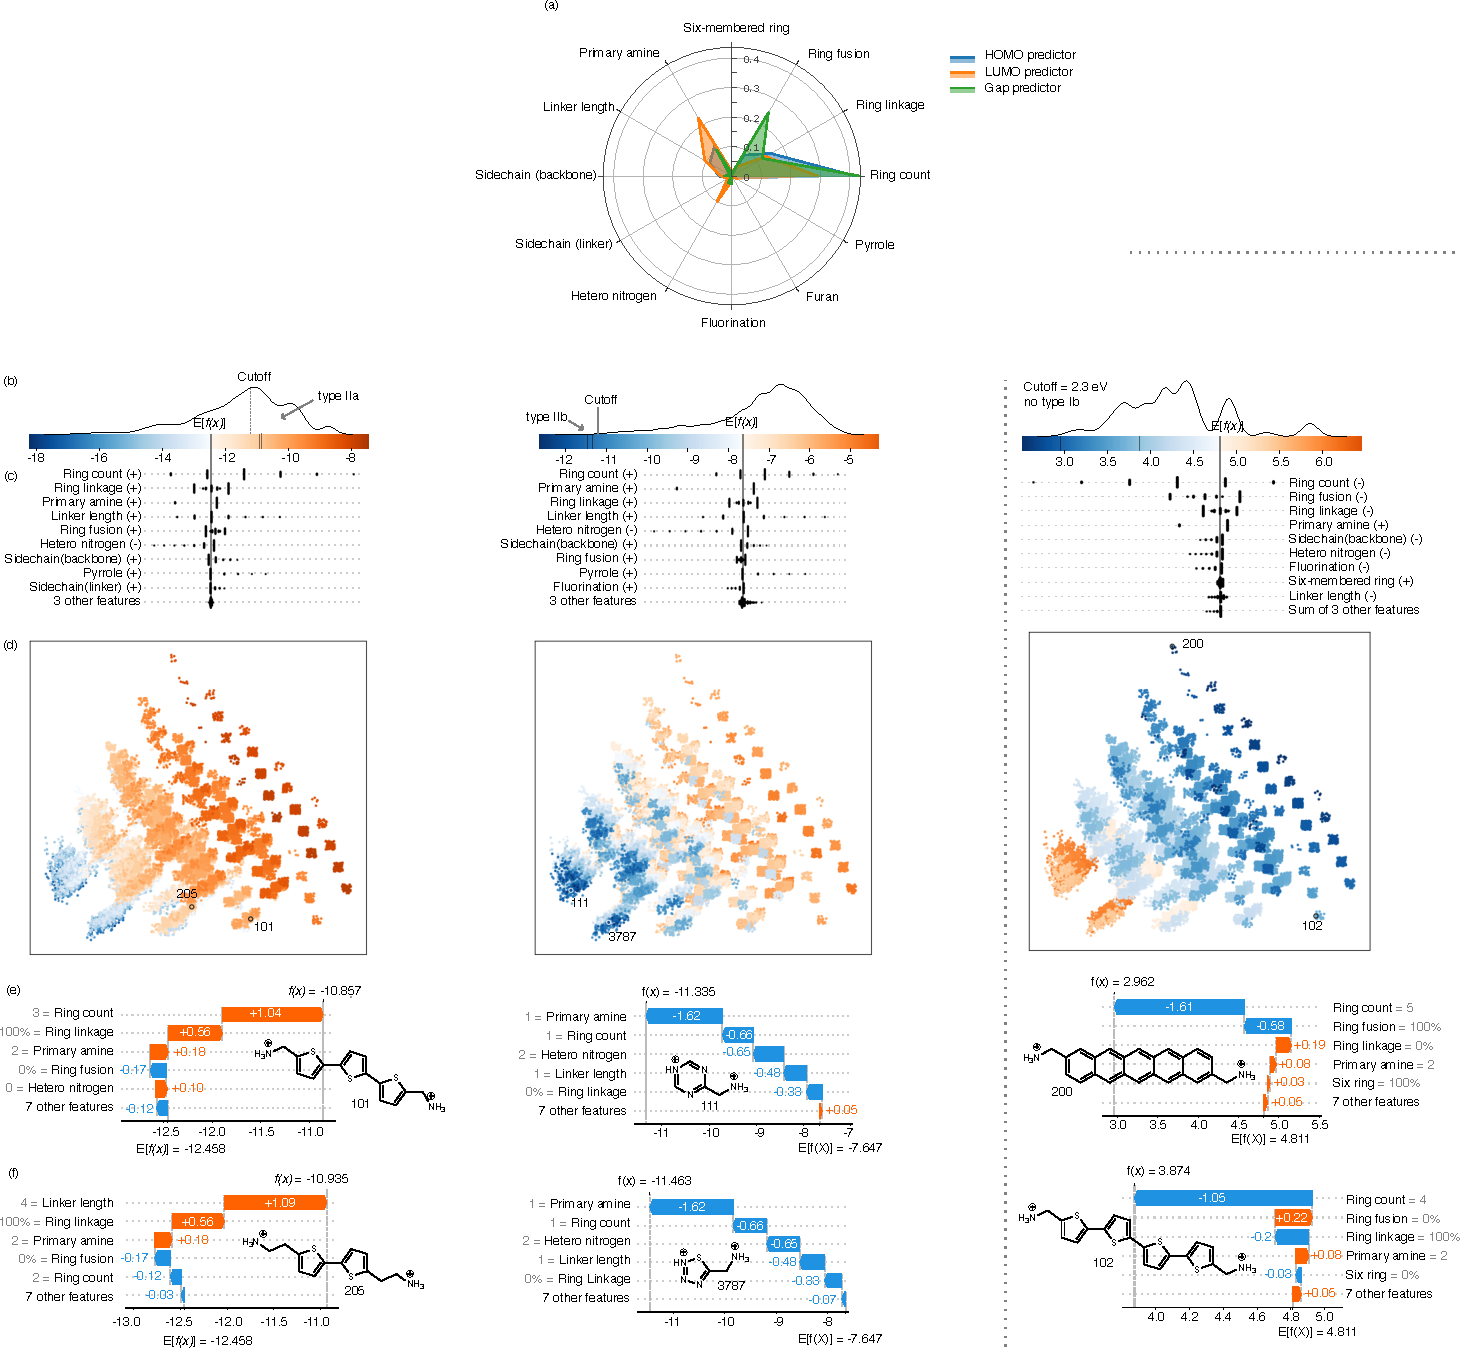
\includegraphics[width=\textwidth]{figures/machine-learning/machine-learning-4.pdf}
\caption[Prediction of organic frontier levels using machine learning.]{Prediction of organic frontier levels using machine learning. (a) Normalized mean absolute SHAP value of 12 organic descriptors for three machine learning models. The three columns in the lower panel represent HOMO, LUMO, and Gap predictors, respectively. Taking the HOMO predictor as an example: (b) Distribution of the predicted HOMO of organic molecules using kernel density estimation. Organic molecules above the HOMO cut-off (-11.20 eV) are estimated to exhibit type IIa energy level alignment. Two vertical lines on the colorbar represents two representative molecules (e, f). (c) Distribution of Shapley values for all features in HOMO predictor. Features are reported on the vertical axis and sorted from the most relevant (i.e., mean absolute SHAP value) at the top to the least relevant at the bottom. Features with a positive relationship with output are labelled as (+) and vice versa. E[f(x)] is the average HOMO value (-12.458 eV). (d) Chemical space map color-coded by value of predicted HOMO. (e, f) Shapley values for two representative organic molecules.}
\label{f:machinelearning4}
\end{figure}

\begin{figure}[!ht]
\centering
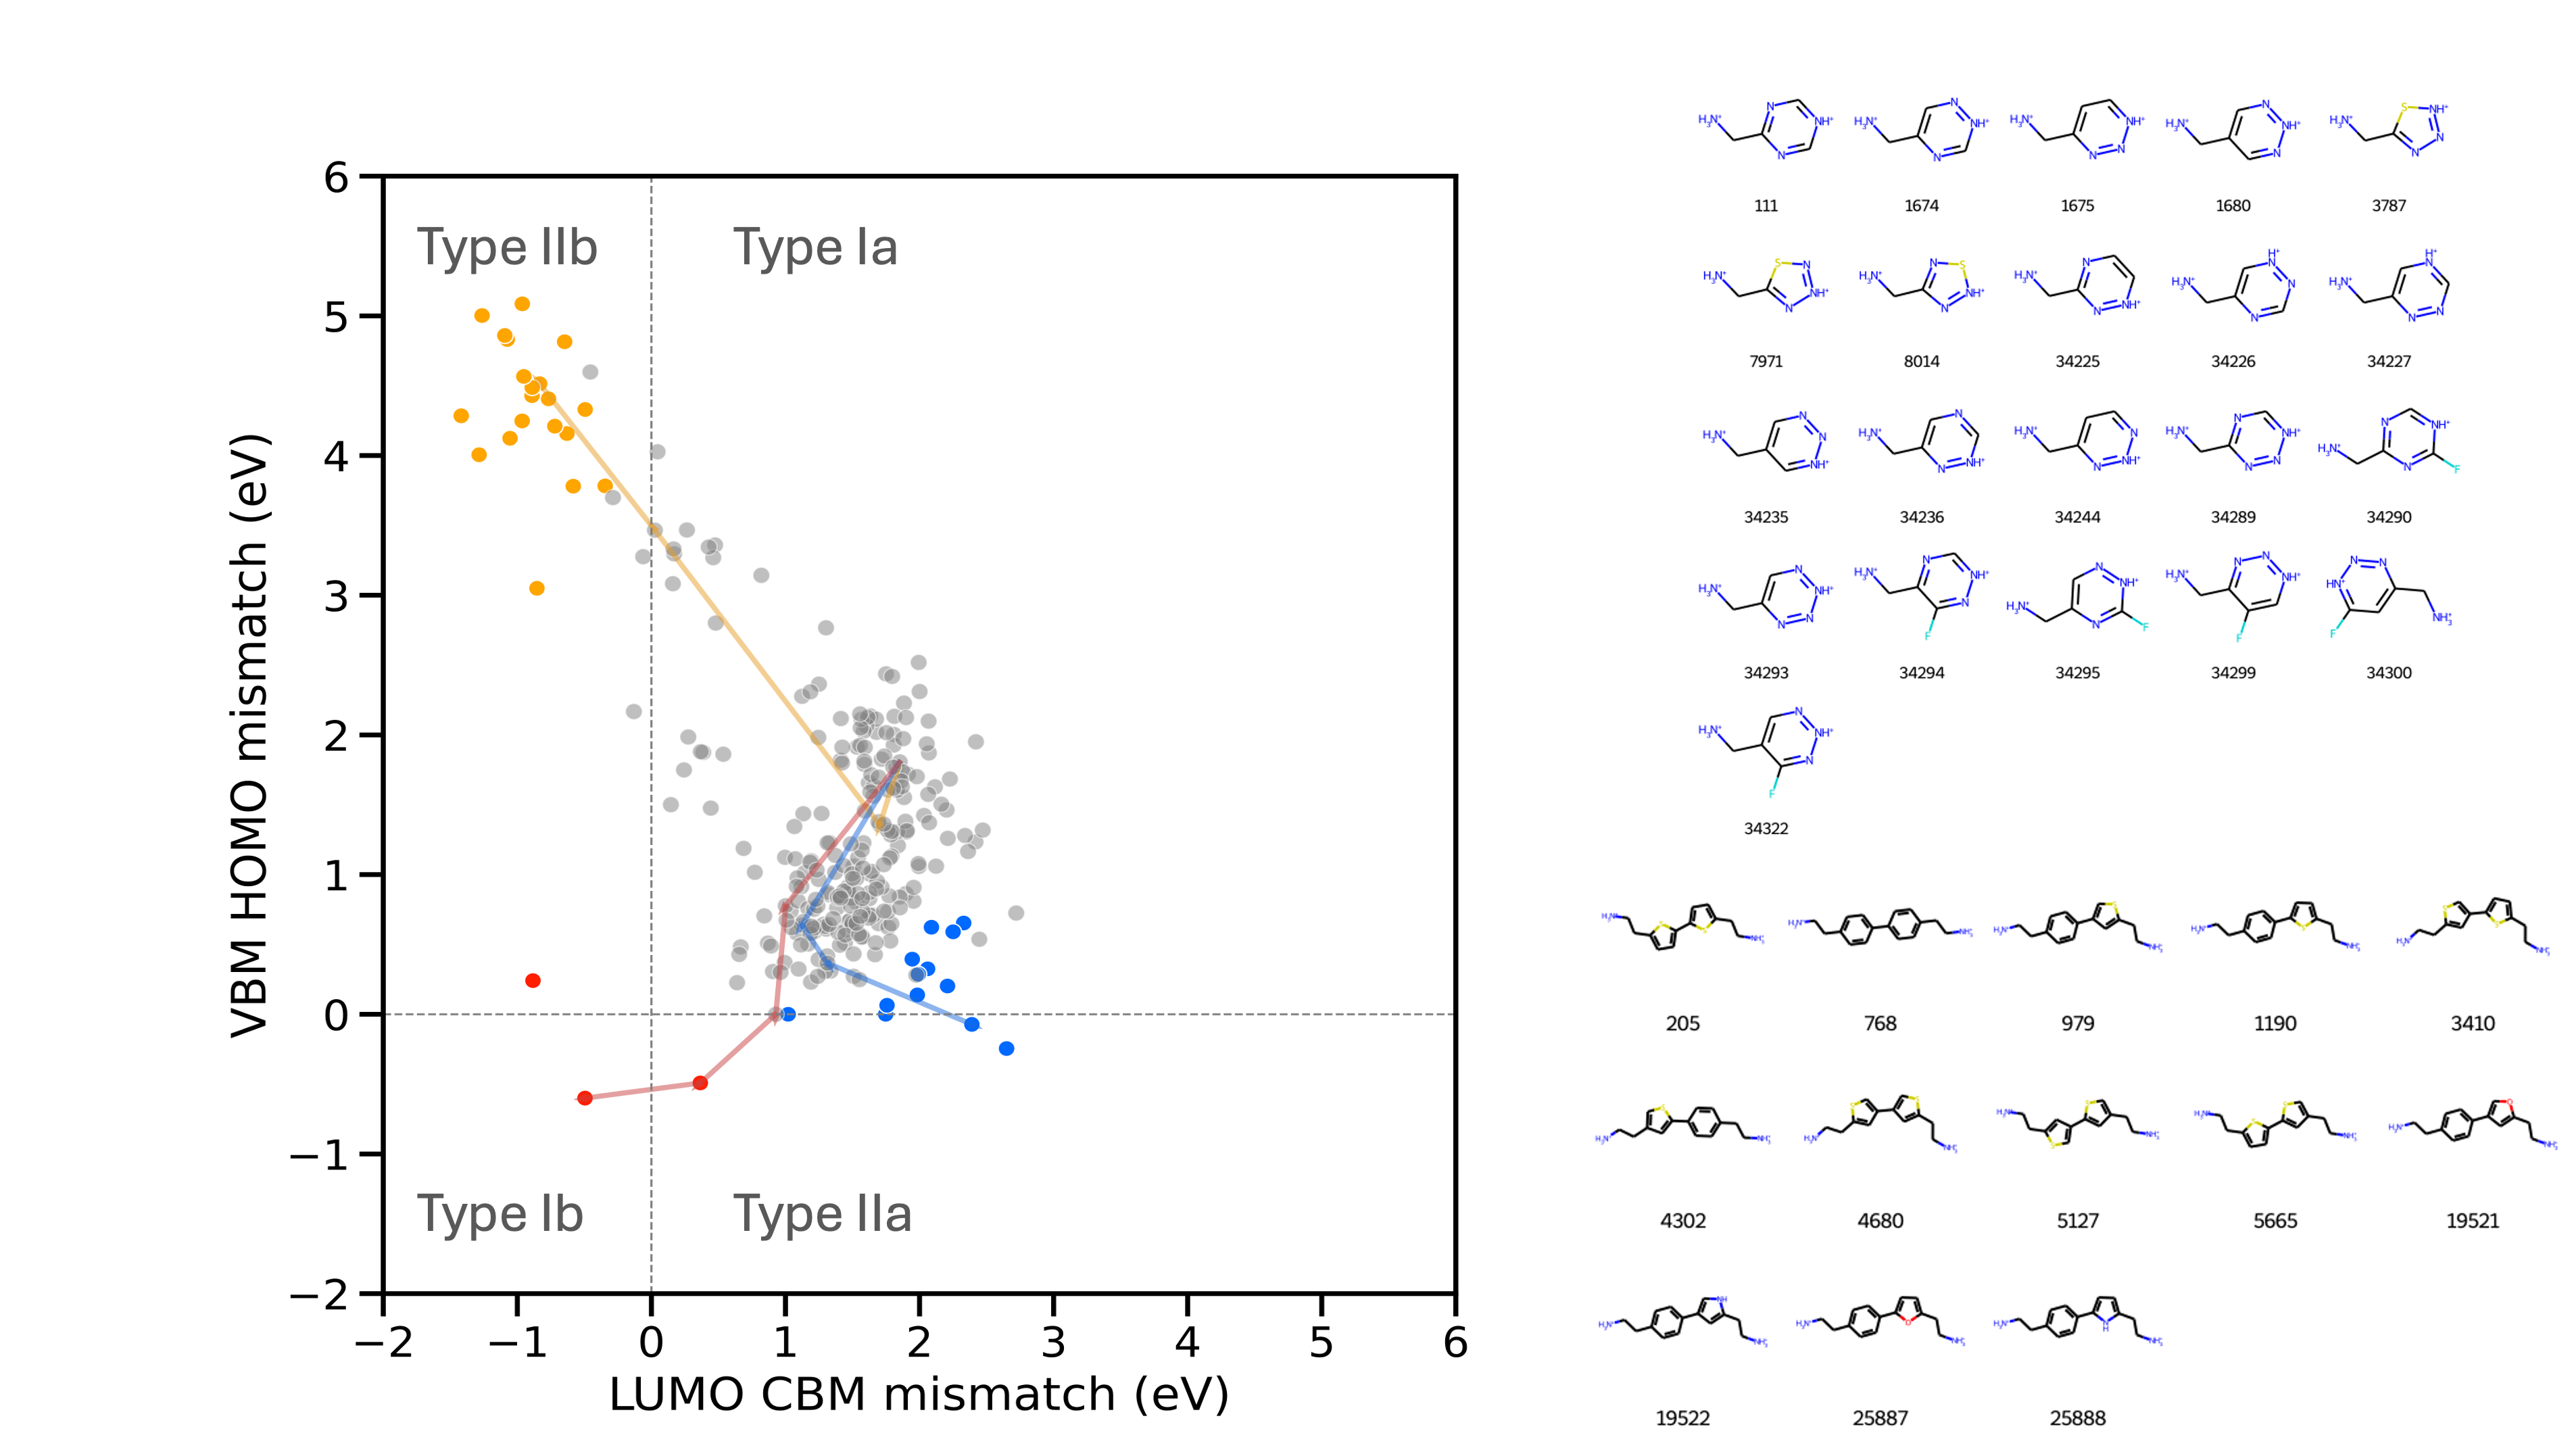
\includegraphics[width=\textwidth]{figures/machine-learning/machine-learning-3.png}
\caption[Organic spacer candidates exhibiting type $II_a$, type $II_b$, and type $I_b$ alignment suggested by machine learning model.]{Organic spacer candidates exhibiting type $II_a$, type $II_b$, and type $I_b$ alignment suggested by machine learning model. (a)Morphing pathways of organic spacers suggested by machine learning model. (b) molecular structure of organic spacer candidates. }
\label{f:machinelearning3}
\end{figure}

To predict the frontier levels of all molecules in the chemical space, we trained three linear models on HOMO, LUMO, and HOMO-LUMO-gap using organic descriptors as input features, respectively. One important consideration is model accuracy. The three models achieve average train/test scores of 0.95, 0.95, and 0.80. The gap predictor’s decreased accuracy is attributed to the challenge of fully capturing the connectivity and conformational effects of increasing numbers of rings, which significantly impact the HOMO-LUMO gap. Despite this, the trend of gap change among different spacers remains accurate, allowing the gap predictor to provide qualitative physical insights about the relationship between input and output. Another critical consideration is model interpretability, essential for ensuring model transparency and building trust in machine learning. Our choice of simple linear regression models enables us to uncover the relationship between organic descriptors and frontier levels in a way that is comprehensible to human. To understand why the model make certain predictions, we interpreted the model using SHAP (Shapley Additive exPlanations) to quantify the contribution of input (organic descriptor) to the output (frontier levels).

We compared the overall importance of features among three models using normalized mean absolute SHAP value (Fig. \ref{f:machinelearning4}a). The SHAP profiles of HOMO and LUMO predictors are more similar to each other, while the gap predictor presents more distinct SHAP profiles. The most relevant feature with the largest Shapley values is ‘Ring count’, as increasing number of rings contribute to higher degree of pi-conjugation, which decrease the separation between organic frontier levels. Additionally, the other two features related to geometry of conjugated pi-orbitals, namely ‘Ring fusion’ and ‘Ring linkage’ also shows importance with all three predictors. ‘Primary amine’, ‘linker length’ and ‘hetero nitrogen’ also plays an important role for HOMO and LUMO predictor, as they are related to the electron richness of the organic molecules, which can shift the frontier levels without changing the gap.

Taking the HOMO predictor as an example, achieving a type IIa energy level alignment requires the HOMO to be above -11.20 eV, with contributions from all features adding up to create a positive overall deviation of the model output from the average value of -12.46 eV. The most important feature for this, quantified by mean absolute SHAP value, is ‘Ring count’ (Fig. 2c). The chemical space map in Fig. \ref{f:machinelearning1}d demonstrate a clear trend showing an increase in HOMO with the number of rings. In the generated chemical space, type $II_a$ candidates are abundant (16,752 out of 35,250), with most being organic spacers featuring three or more rings. These instances exhibit a substantial contribution from the ‘Ring count’ feature, leading to HOMO values close to the cut-off, as exemplified in Fig. \ref{f:machinelearning1}e. Some 2-ring organic spacers may also meet the type $II_a$ criteria, with other features making key positive contributions, such as linker length in Fig. \ref{f:machinelearning1}f. Type $II_b$ candidates, characterized by a LUMO below the cut-off of -11.20 eV, are less common (53 out of 35,250), as the cut off is significantly smaller compared to the average LUMO at -7.65 eV. For these organic spacers, all features must be at specific values to produce a maximized negative deviation in the model output. These spacers are less diverse, typically feature one ring, one primary amine, no more than 1 carbon for linker length, and hetero nitrogen substitution, as exemplified in Fig. \ref{f:machinelearning1}. In contrast, the type Ib alignment is the least common (0 out of 35,250), requiring a HOMO-LUMO-gap below 2.3 eV.  

